\documentclass[CMPE]{../KGCOEReport}
\usepackage{float}
\usepackage{adjustbox}
\graphicspath{ {./images/} }

\newcommand{\exerciseNumber}{2}
\newcommand{\exerciseDescription}{Register File}
\newcommand{\dateDone}{February 22, 2024}
\newcommand{\dateSubmitted}{February 25, 2024}

\newcommand{\name}{Mohammed Fareed}
\newcommand{\classCode}{CMPE 260}
\newcommand{\LabSectionNum}{4}
\newcommand{\LabInstructor}{Prof.\ Richard Cliver}
\newcommand{\TAs}{Aubrey Tarmu \\ Henry Bang \\ William Tom}
\newcommand{\LectureSectionNum}{2}
\newcommand{\LectureInstructor}{Prof.\ Marcin Lukowiak}

\begin{document}
\maketitle

\section*{Abstract}

In this exercise, the design, implementation, and verification of a register file within a Field Programmable Gate Array (FPGA) environment were done, utilizing the Xilinx Vivado Design Suite. The primary focus was the creation of a digital system capable of storing and accessing multiple words, employing a two-read, one-write configuration. The project began with the specification of the register file, designed to support parallel data retrieval from two addresses, enhancing data access speed. Initial testing was conducted through behavioral simulation, ensuring the system's functionality met predefined specifications. This was followed by synthesis and post-implementation timing simulations, assessing the design's performance and identifying potential delays inherent to FPGA operations. The exercise also involved a hardware demonstration on a Basys3 FPGA platform. The results verified the register file's operational integrity and compliance with design requirements.

\section*{Design Methodology}

The register module is the basic building block of our project, designed to store bits of digital information within the FPGA. A "2-D Array" structure was used for these modules to organize data storage and access.
The number and size of the registers was parameterized, using the following constants in a global package:

\begin{itemize}
    \item \verb|BIT_DEPTH|: The size of the data bus (register size).
    \item \verb|LOG_PORT_DEPTH|: The address bus size (\(\log_2\)(number of registers)).
\end{itemize}

The register file combines these modules into a system that allows for parallel data access, adopting a two-read, one-write approach. This setup significantly improves the efficiency of data retrieval, reducing the time required for retrieving instruction operands and enhancing the system's overall performance.

The system's operation is controlled by various input signals:

\begin{itemize}
    \item \verb|clk_n|: Falling edge-triggered clock signal.
    \item \verb|we|: Write enable signal.
    \item \verb|Addr1|, \verb|Addr2| (\verb|LOG_PORT_DEPTH| wide): Address lines for reading data.
    \item \verb|Addr3| (\verb|LOG_PORT_DEPTH| wide): Address line for writing data.
    \item \verb|wd| (\verb|BIT_DEPTH| wide): Data to be written to the register file.
\end{itemize}


The \verb|clk_n| signal, ensures that data writing and reading are synchronized. The write enable (\verb|we|) signal allows data to be written to the registers, protecting against accidental data loss. Two address lines (\verb|Addr1| and \verb|Addr2|) are used for reading data, while a third address line (\verb|Addr3|) is used for writing data. The data to be written is specified by the \verb|wd| signal. The register file has the following outputs:

\begin{itemize}
    \item \verb|rd1|, \verb|rd2| (\verb|BIT_DEPTH| wide): Data read from the register file.
\end{itemize}

The \verb|rd1| and \verb|rd2| signals output the data read from the register file at the addresses specified by \verb|Addr1| and \verb|Addr2|, respectively.
\\

A specific feature of the design is making register 0 immutable, meaning it always outputs zero. This decision ensures a constant zero value is available for computations requiring it, thus adding to the system's functionality.

\section*{Results and Analysis}

The register file was implemented using VHDL, with the global constants defining the register size and address bus size to be 32 bits and 5 bits, respectively. The design was tested using behavioral simulations, ensuring the system's correct operation. Synthesis and post-implementation timing simulations were then performed to assess the design's performance of FPGA operations.
The following are all the test cases that were run on the register file:

\begin{table}[h]
\centering
\begin{tabular}{|c|c|c|c|c|c|c|}
\hline
we & Addr1 & Addr2 & Addr3 & wd & RD1 & RD2 \\
\hline
'0' & 000 & 000 & 001 & 10 & 00 & 00 \\
'1' & 000 & 000 & 001 & 10 & 00 & 00 \\
'1' & 001 & 000 & 010 & ff & 10 & 00 \\
'0' & 010 & 011 & 100 & 20 & ff & 00 \\
'1' & 011 & 100 & 101 & 33 & 00 & 00 \\
'0' & 100 & 101 & 110 & 44 & 00 & 33 \\
'1' & 101 & 110 & 111 & 55 & 33 & 00 \\
'1' & 110 & 111 & 000 & 66 & 00 & 55 \\
'1' & 111 & 000 & 001 & 77 & 55 & 00 \\
'0' & 000 & 001 & 010 & 88 & 00 & 77 \\
\hline
\end{tabular}
\caption{Simulation Test Cases.}
\label{tab:test_cases}
\end{table}

The test cases in Table \ref{tab:test_cases} were run on the register file, with assert statements to ensure the correct operation of the design. The test cases mainly focus on testing the operation of the \verb|we| signal, correctly reading data from the register file after writing to it, and ensuring that register 0 can't be written to, always returning zero.\\

The results of the simulations were observed to ensure the register file's correct operation and timing. Figure \ref{fig:behavior} shows the behavioral simulation results of the register file.

\begin{figure}[H]
    \centering
    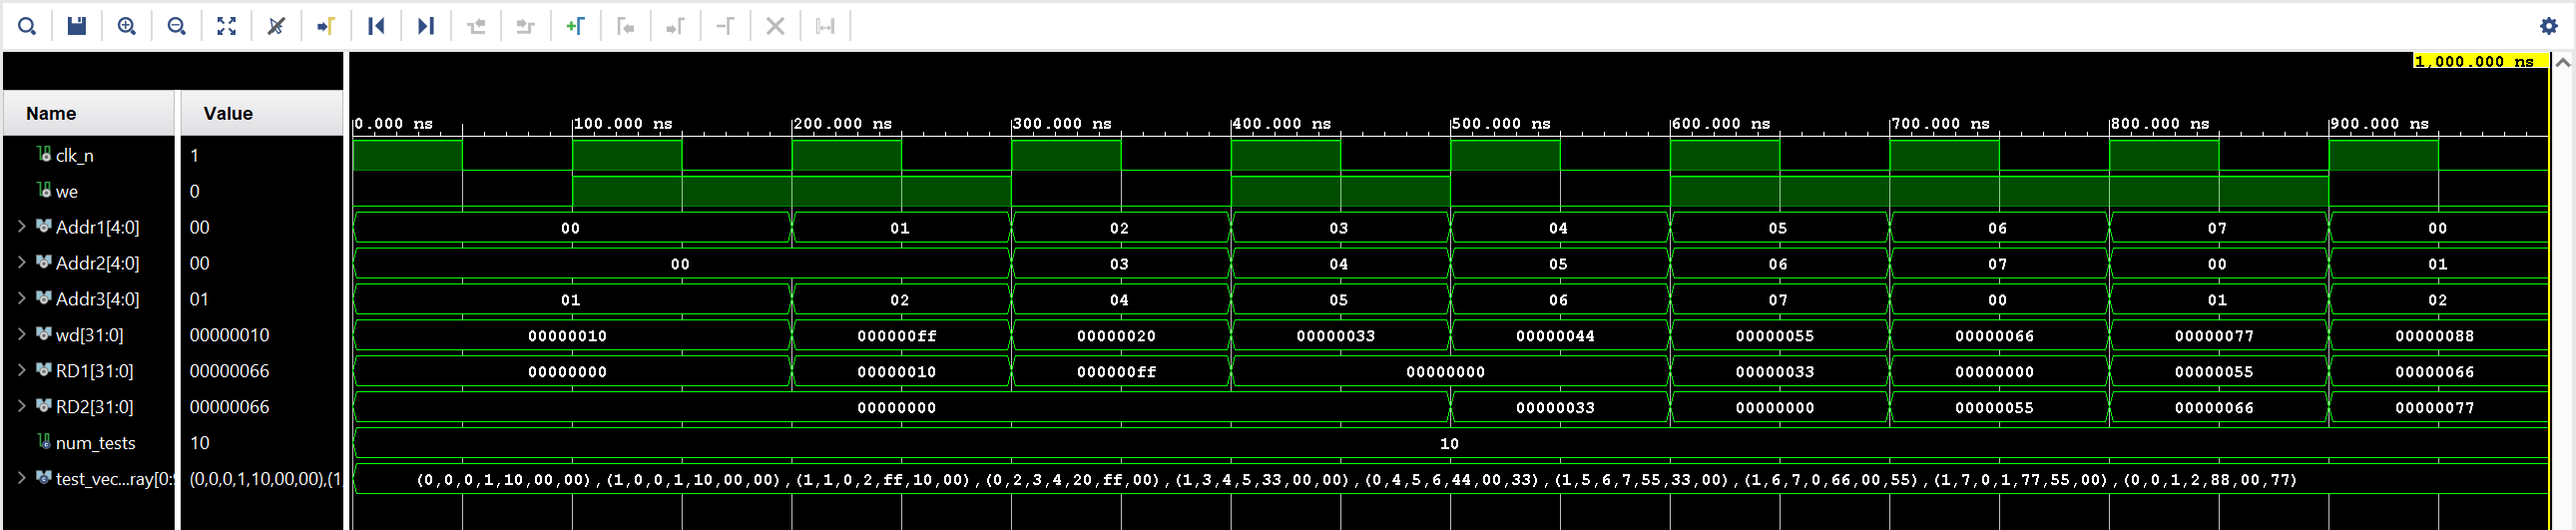
\includegraphics[width=1\textwidth]{behavior.png}
    \caption{Behavioral Simulation Results.}
    \label{fig:behavior}
\end{figure}

The figure above shows the behavioral simulation results of the register file, with the input and output signals labeled. The simulation results demonstrate the correct operation of the register file, with the read data matching the written data. The simulation results also show the read data being zero when the address is zero, as expected. It also shows th e data \verb|0xff| to address 2, then reading from address 2, which correctly returns \verb|0xff|.\\

The register file was then implemented on a Basys3 FPGA, and the design was verified through a post-implementation timing simulation. Figure \ref{fig:implement} shows the post-implementation timing simulation results of the register file.

\begin{figure}[H]
    \centering
    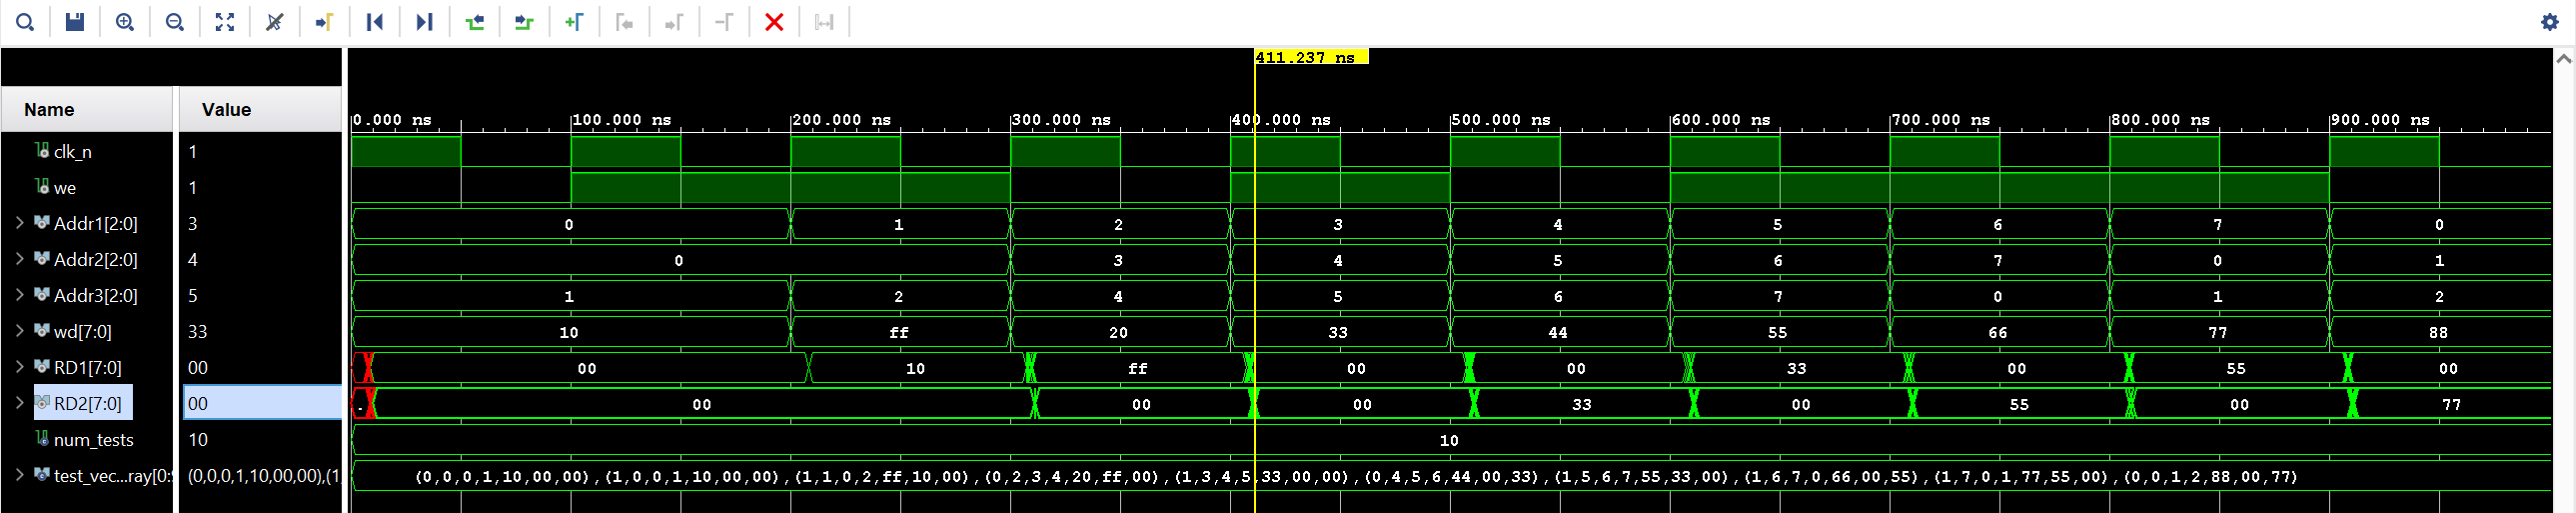
\includegraphics[width=1\textwidth]{implement.png}
    \caption{Post-Implementation Timing Simulation Results.}
    \label{fig:implement}
\end{figure}

The figure above shows the post-implementation timing simulation results of the register file. The simulation results demonstrate the correct operation of the register file, with delays within the expected range, which ensures the design's performance and timing. An average delay of around 11 ns was observed on \verb|rd1| and \verb|rd2| signals, which is within the acceptable range for the design.

The results of the hardware demonstration on the Basys3 FPGA platform verified the register file's operational integrity and compliance with design requirements.

\section*{Conclusion}

The design, implementation, and verification of a register file within a Field Programmable Gate Array (FPGA) environment were successfully completed. The register file was designed to support parallel data retrieval from two addresses, enhancing data access speed. The design was tested using behavioral simulations, ensuring the system's correct operation. Synthesis and post-implementation timing simulations were then performed to assess the design's performance of FPGA operations. The results of the simulations demonstrated the correct operation of the register file, with delays around 11 ns, which are within the expected range, ensuring the design's performance and timing. The hardware demonstration on the Basys3 FPGA platform verified the register file's operational integrity and compliance with design requirements.

\newpage
\begin{figure}[H]
    \centering
    \begin{adjustbox}{center}
        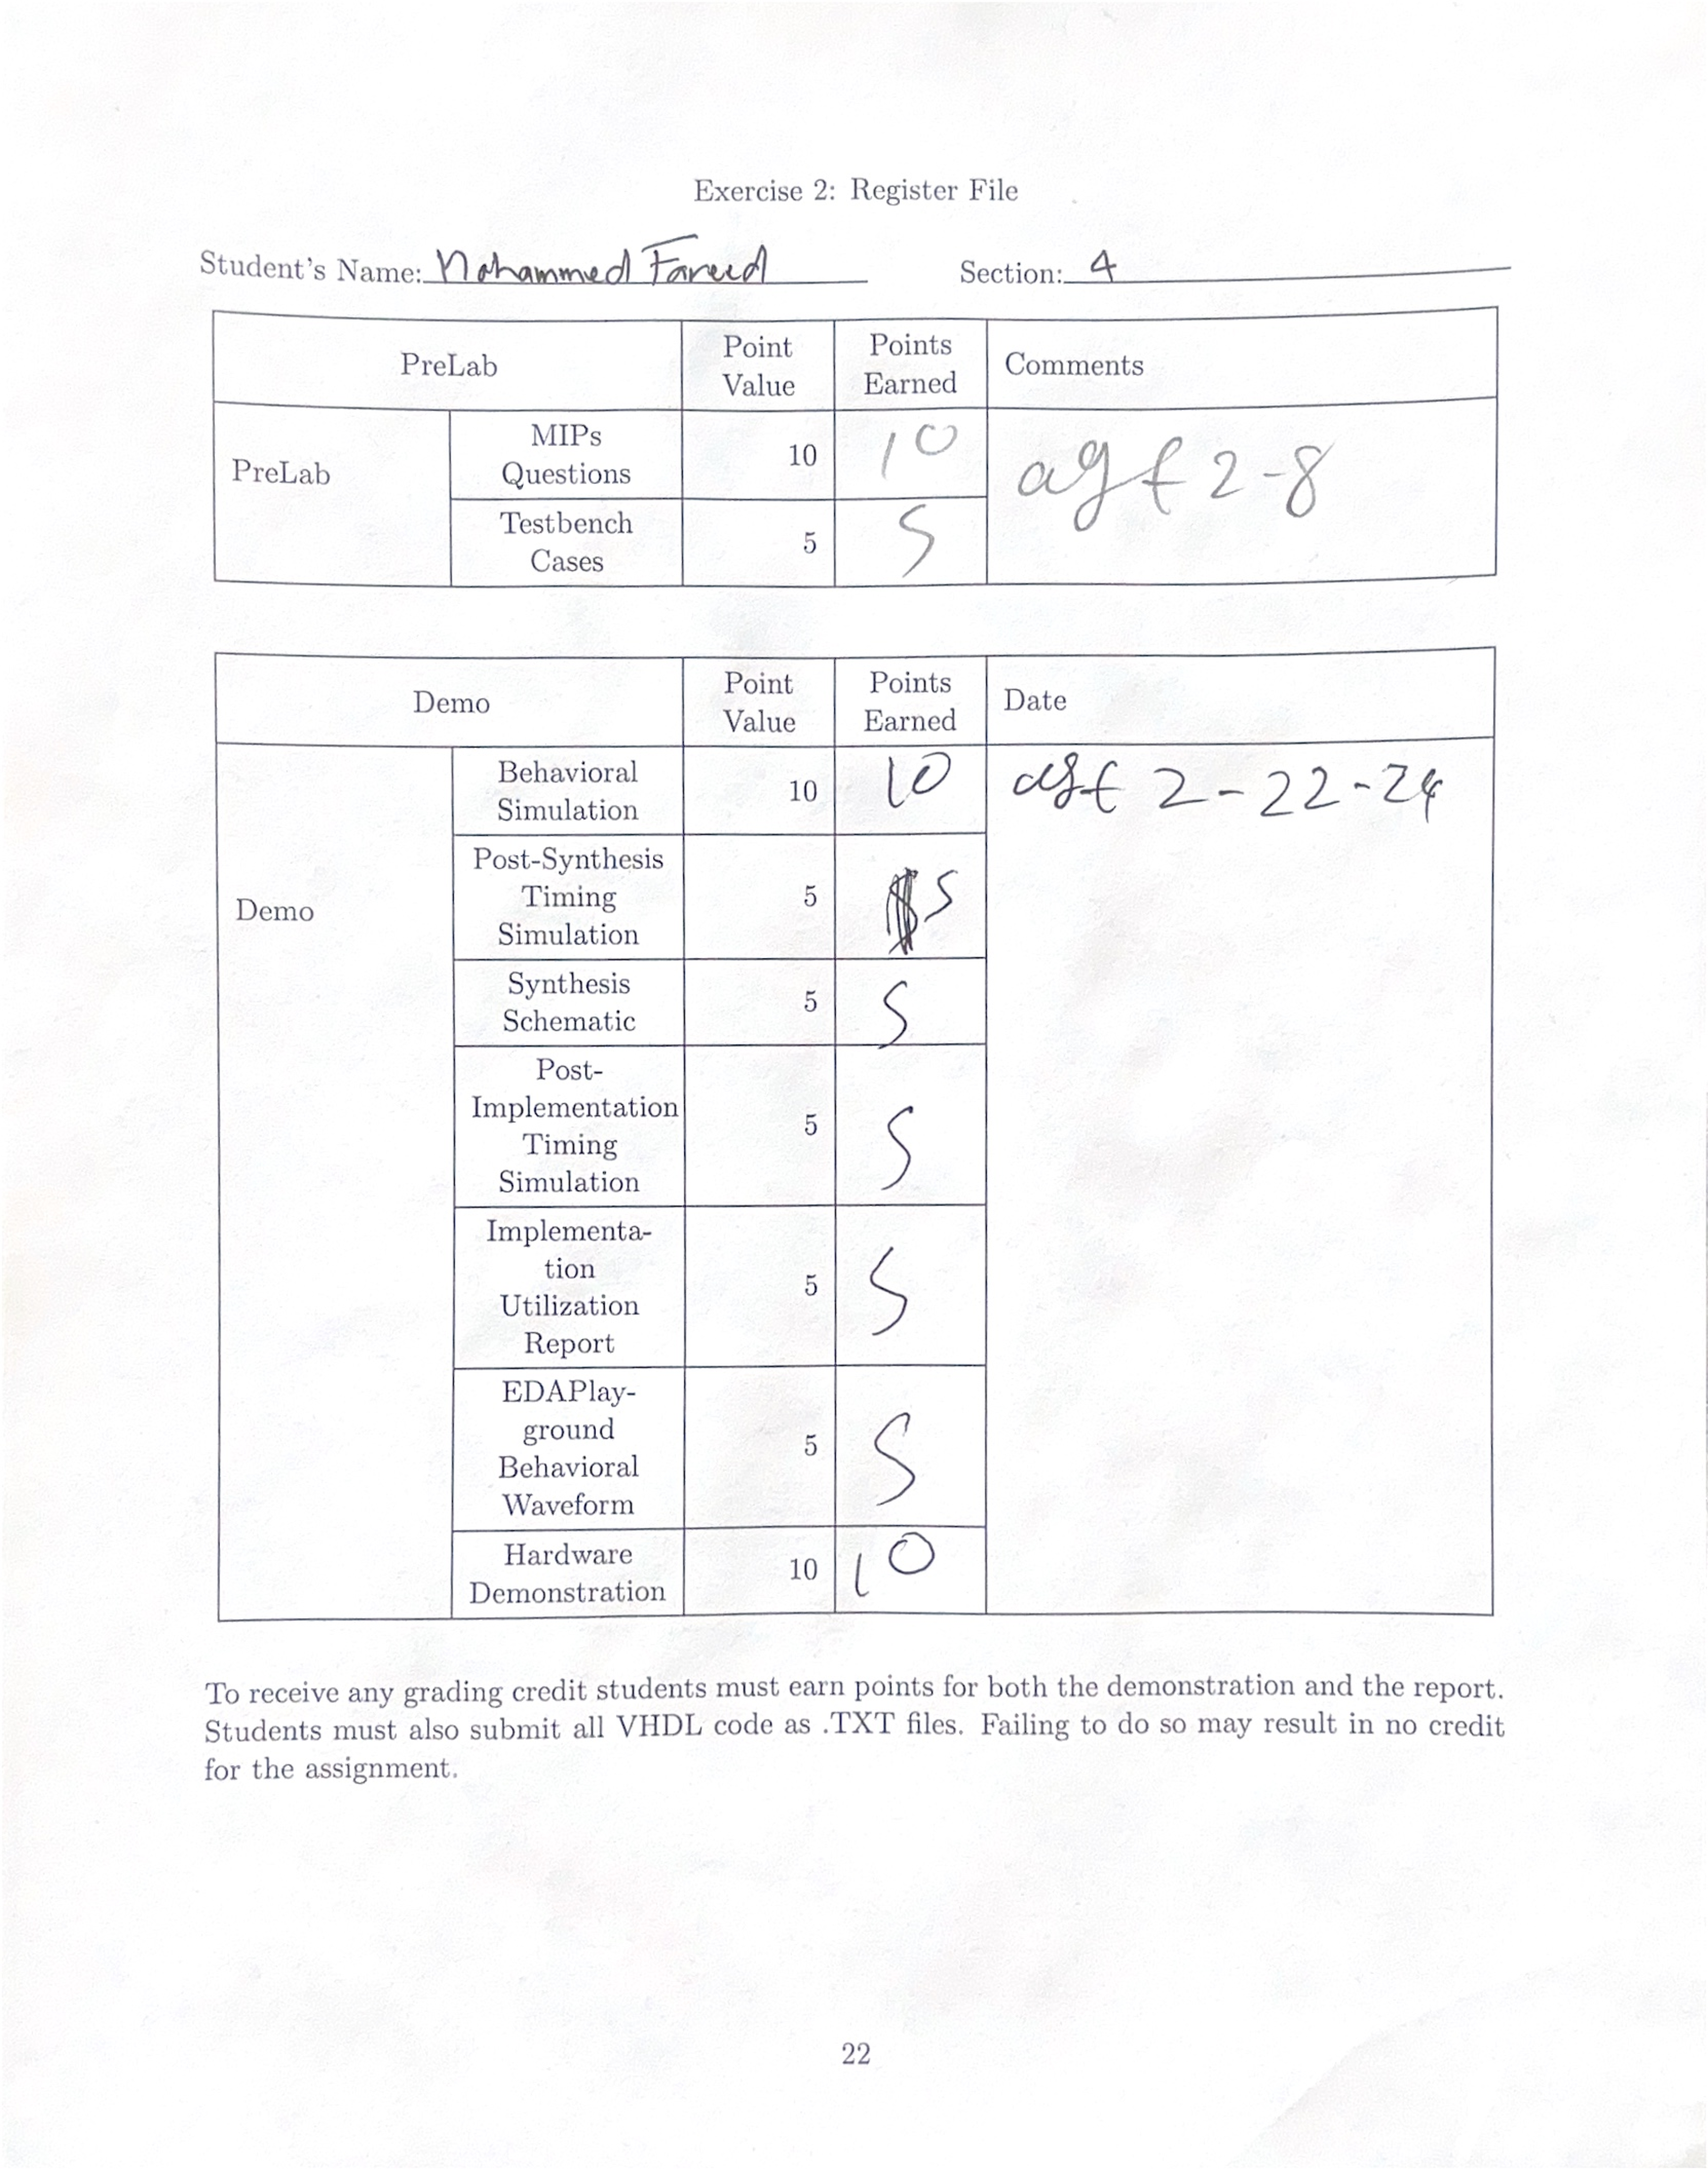
\includegraphics[width=1.35\textwidth]{signoff.pdf}
    \end{adjustbox}
\end{figure}

\end{document}
